\documentclass[a4paper,12pt]{report}

%Packages for timeline
\usepackage{array, booktabs}
\usepackage[x11names,table]{xcolor}
\usepackage{caption}
\DeclareCaptionFont{blue}{\color{LightSteelBlue3}}
\newcommand{\foo}{\color{LightSteelBlue3}\makebox[0pt]{\textbullet}\hskip-0.5pt\vrule width 1pt\hspace{\labelsep}}
%%%%%%%%%%%%%%%%%%%%%%%%%%%%%%%%%%%%%%%%%%%%%%%%%%%%%%%%%%%%%%%%%%%%%%%%%%%%%%%%


\usepackage[utf8]{inputenc}
% \usepackage[Vietnamese]{babel}
\usepackage{titling}
\usepackage{rotating}
%package the indent the first line in latex
\usepackage{indentfirst}
\usepackage{graphicx}
\usepackage{ragged2e}
\usepackage{ragged2e}
\usepackage{afterpage}
\usepackage{amsmath}
\usepackage{subcaption}
\usepackage{float}
\usepackage{alltt}
\usepackage{listings}
%adding bibliography
\usepackage[backend=biber]{biblatex}
\addbibresource{/home/pj/MEGA/ComVi/paper_writing/Mendeley/bibitex/library.bib}

\graphicspath{{/home/pj/Documents/proposal/}}
% \graphicspath{{~/coding/python/Music-Sheet-Pitch-Translation/Latex_paper/draft}}

%making the numbering in Roman format 
\renewcommand\thesection{\Roman{section}}
\renewcommand\thesubsection{\roman{subsection}}

\setlength{\droptitle}{-8cm}

\usepackage{tikz}

%for table at the end of the proposal
% \usepackage{booktabs}   Dont use booktab the traditional method is still better
\usepackage{tablefootnote}
\usepackage{footnote}
\usepackage{multirow}
\usepackage{graphicx}
%  \usepackage[table,xcdraw]{xcolor}

\pretitle{
    \begin{tikzpicture}[remember picture,overlay]
    \node[anchor=north west,yshift=-1.5pt,xshift=1pt]%
        at (current page.north west)
        {\includegraphics{vgu_logo}};
    \end{tikzpicture}
}
\posttitle{}

\begin{titlepage}
	\title{ MUSIC SHEET UNDERSTANDING AND TONES TRANSPOSITION}
	\author{}
\end{titlepage}


\begin{document}

\afterpage{\null\newpage}

\maketitle

\tableofcontents

\clearpage

\section{Research team members}
\begin{itemize}
	\item Team Leader:      \hfill Truong Minh Khoa  (VGU CSE 2018)
	\item Team Member: 		\hfill Dinh Cong Minh (VGU CSE 2019)
	\item Team Member:	    \hfill Nguyen Tho Anh Khoa (alumni of HCM University of 

                            \hfill Technology K14)
	\item Team Member:	    \hfill Huynh Minh Triet (VGU CSE 2019)
    \item Supervisor        \hfill Dr.Dinh Quang Vinh,CSE (Faculty of VGU) 
\end{itemize}


\section{Disclaimer} 
This report is a product of our team's work, unless otherwise referenced. In
addition, all opinions, results, conclusions, and recommendations are of our own
and may not represent the policies or opinions of the Vietnamese-German
University's Department of Engineering or the University as a whole. 

\clearpage

\section{Abstract} 

The field of Optical Music Recognition (OMR), a subfield in Artificial
Intelligence, is aimed at automating the translation or understanding of music
sheets \cite{Calvo-Zaragoza}.  However, there is a lack of applications to solve
the problem of musical tones transposition (the process of moving a collection
of notes up or down in pitch by a constant interval).  Such a problem in tones
transposition is highly labor-intensive if the musician has to reorder the notes
manually, often impossible if done during a performance. Our work proposes a way
in which musicians can perform tones transposition by scanning a music sheet,
input the number of shift tones or semitones required, and then the programm
will output an audio file or a new music sheet with all of the notes shifted to
the required pitch. 

% \section{Team's workload}
% Due to the nature of our work is in pure code I believe the best way to show how 
% much each member contribute to the project can be directly viewed via our github
% commit page:



\section{Introduction}

The topic of recognizing musical sheets, i.e., Optical Music Recognition (OMR),
is not a novel field of research. The term OMR first appeared in a paper written
by MIT scientists in the 60s.  During the last three decades until now, OMR is
an ever increasingly developing field and is capable of solving many problems
that involve music \cite{Shatri2020a}\\

More specifically, the current OMR systems of today are capable enough to
recognize a printed musical sheet and digitize it. The resulting output could be
a .midi file, or other types of sound files such as .way, .mp3. The vast
majority of those researches are dedicated to the common user, even for users
who are not educated on musical theory, but there is still a lack of products
that can be used by professional or enthusiast musicians. In reality, a common
problem that is encountered is the transposition of music tones, i.e., shifting up or down a constant interval of
semitones or tones for the whole music sheet. Currently to obtain a music
sheet with a few tones higher or lower the musician has to manually retype the
entire musical sheet by hand, which is labor-intensive and time-consuming.


\clearpage

\section{Proposed Method}
The process includes the first stage, Staff Line Preprocessing, to remove the
lines on each staff for ease of musical note detection. The second stage is Note
Translation to translates the detected notes into scientific pitch notation. The
third stage, Tone Transposition will transpose the semitones or tones of the
song to give the final output. 

\subsection{Staff Line Preprocessing}
For ease of note recognition, first, the staff lines must be detected and
removed. This process includes two stages. First, detection of the staff lines
and their thickness; second, removal of those staff lines.

\subsubsection{Staff Line Detection}
To detect the staff line in the music sheet we first need to remove all of the notes.
This is done for ease of staff line detection.\\

Our staff's line detection algorithm will first grayscale the image and then
invert the image colors so that the lines are now white and the background is
black. The color inverted music sheet is then run with the OpenCV built-in
dilate() function, where the horizontal lines will be expanded so that its width
is increasingly larger, and any white pixels, i.e., notes, that does not belong
to the horizontal line, will be flipped to 0 and becomes the background thus
eliminating all of the notes.\\

% \clearpage
Result:
\begin{figure}[H]
    \centering
    \begin{subfigure}[t]{0.5\textwidth}
        \centering
        \includegraphics[height=2.0in]{b4_dilate}
        \caption{before applying dilate function}
    \end{subfigure}%
    ~ 
    \begin{subfigure}[t]{0.5\textwidth}
        \centering
        \includegraphics[height=2.0in]{after_dilate}
        \caption{after applying dilate function}
    \end{subfigure}
\end{figure}

The dilated image above will give an output that is fairly accurate except for a
few lines at the last staff line. This is why we then use \textcite{Gomez2017}'s
method and Run Length Encoding (RLE) to determine the lines' thicknesses and
their distance between one another. RLE will be applied vertically along a
random column of the dilated image above:\\

\begin{figure}[ht]
\makebox[\textwidth]{\includegraphics[scale = 0.5]{apply_RLE}}
\caption{dilated image after running RLE on a random column \protect\footnotemark }
\label{}
\end{figure}

\footnotetext{This image was taken from \textcite{Gomez2017} which was done on a
note removed but not color inverted music sheet. Which is why the line is in
black and the distance is in white, opposite to our dilated image.}

RLE will group adjacent pixels of the same color into one group with a number to
indicate how many pixels of the same color is within that group and a character
to indicate that group is either a group of black pixels "B" or a group of white
pixels "W". Through which the staff line thickness and the distance between two
staff lines are then obtained. More specifically, to extract the distance between each
staff line, e.g., our RLE output might be 3B,2W,4B,2W,3B,3W,3B,2W, the black
group (because our music sheet is color inverted so black is the distance) that
appear most often "3B" with the value of three pixels is chosen. Therefore, the
distance between two staff lines is three pixels. The same method is also applied
to get the thickness of the lines.

\subsubsection{Staff Line Removal}
In our music sheet, places where there is only lines will have matrix of 
this type:

\begin{figure}[ht]
    \centering
    $
\begin{pmatrix}
	0 & 0 & 0\\
	1 & 1 & 1\\
	0 & 0 & 0
\end{pmatrix}
$\\
\caption{an example of a kernel with only line and no notes}
\label{line only matrix}
\end{figure}

\medskip

Please note that the rows of ones represent the thickness of the line, which can
vary from one to multiple rows, the same thing goes for the row of zeros, distance
between each line.

\begin{figure}[h]
    \makebox[\textwidth]{\includegraphics[width=\linewidth]{inverted_two_staves.png}}
    \caption{The current color inverted music sheet}
    \label{}
\end{figure}
 
To remove the staff lines on each music line, a check vector of length N will be run 
on each NxN kernel of the image:\\

\begin{figure}[ht]
    \centering
$
\begin{pmatrix}
	1 & ... & 1 & 0 & ... & 0 & 1 & ... & 1
\end{pmatrix}
$\\
\caption{Check vector of length N}
\label{check vector}
\end{figure}

The number of ones and zeros in figure \ref{check vector} depends on
the thickness of each line and the distance between two staff lines
respectively, which was obtained in the previous section.  For example, with the
kernel in figure \ref{line only matrix} the check vector will be of the type:

\begin{figure}[h!]
    \centering
    $
    \begin{pmatrix}
       1 & 0 & 1 
    \end{pmatrix}
    $\\
\end{figure}

 This check vector is then multiplied with every NxN kernel of the image. If the
 kernel is of the type of a line, the result will be a vector of 0s, otherwise,
 the vector result will contain at least one positive integer among its
 elements.\\

 For every time we encounter an area that is a line by using the check vector,
 the found area will be replaced by the NxN matrix which is full of 0s, else it
 will be ignored and we will continuously check the next kernel. The process
 will be terminated when we have checked all the possible kernels in the
 image.\\

\clearpage
Finally, inverting the color of the output image one last time will result in a
music sheet with lines removed:
\begin{center}
  \makebox[\textwidth]{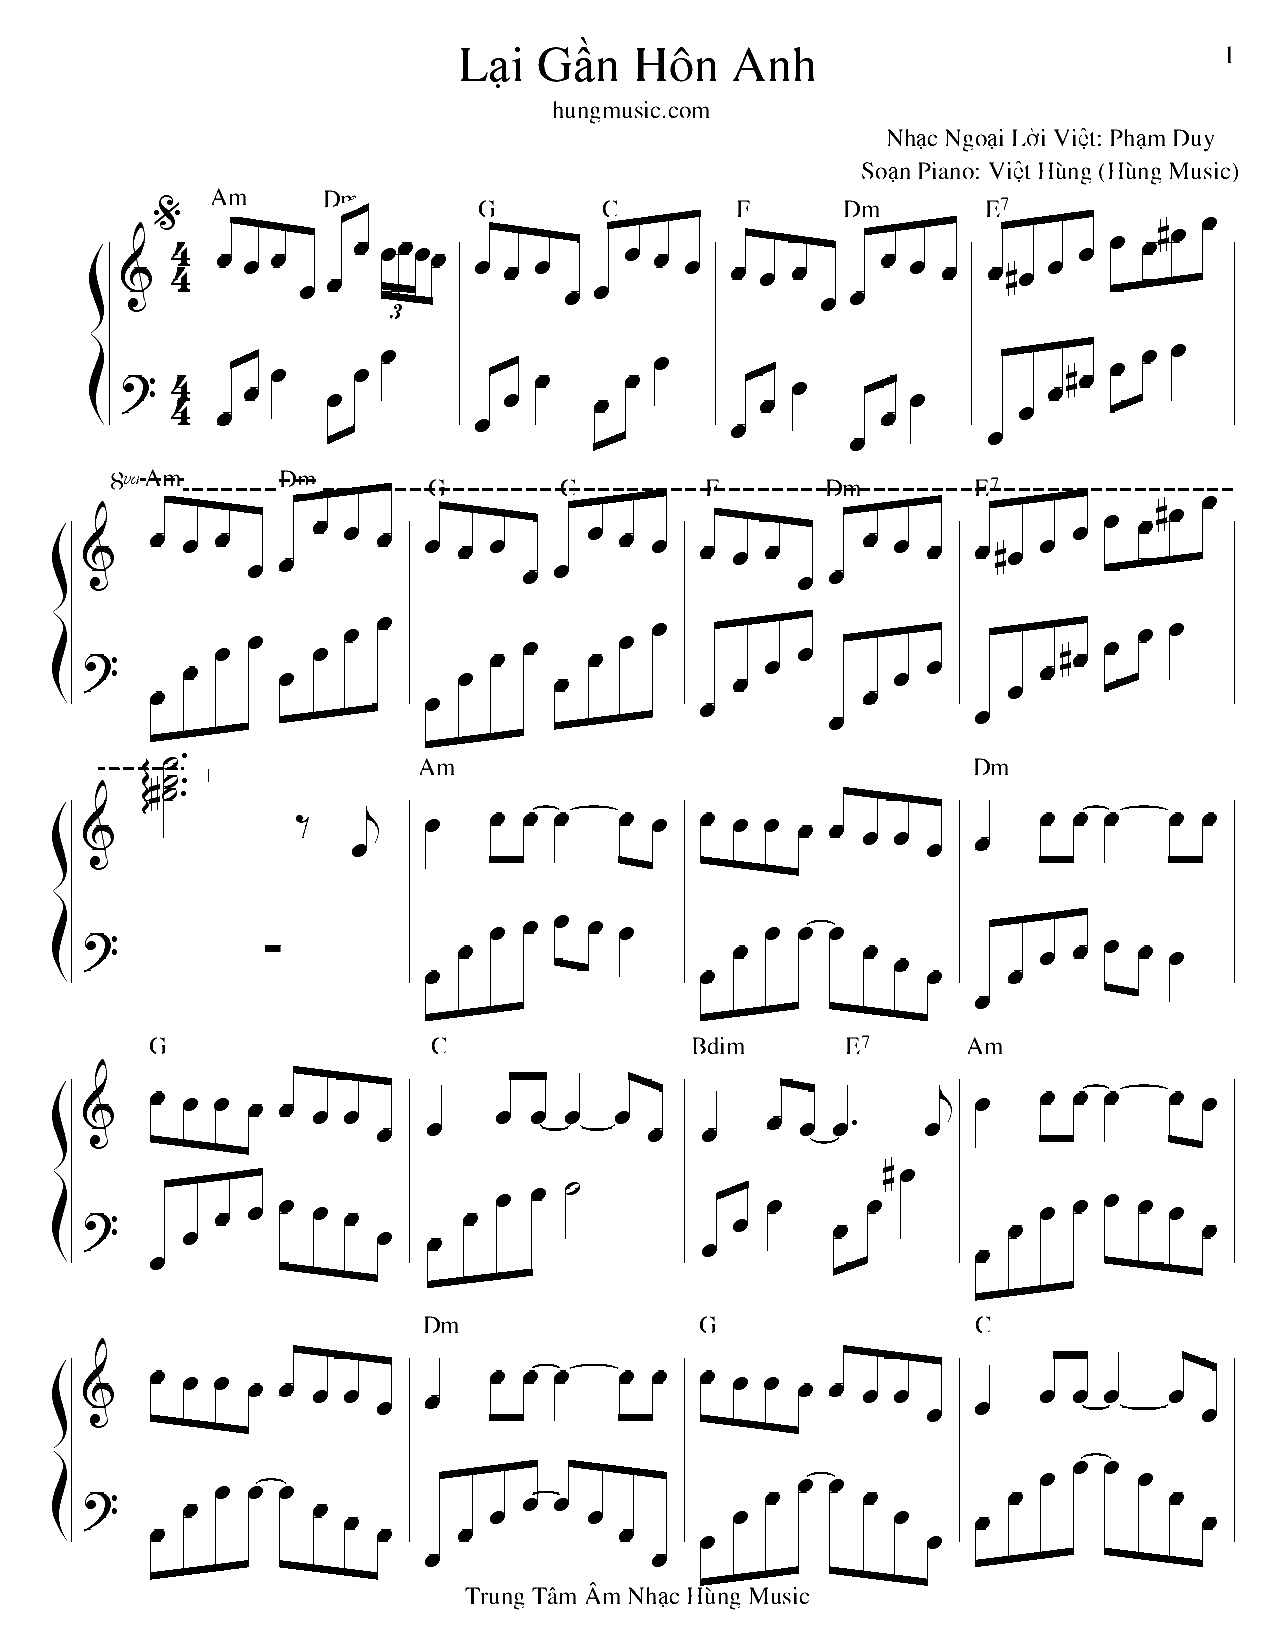
\includegraphics[width=\linewidth]{staffRemoval.jpg}}
\end{center}

\clearpage

\subsection{Note Translation}

To translate the note from its input as pictorial data to scientific pitch
notation so that the computer can process the music sheet, three steps are
required. First by using \textcite{Rosebrock} method to eliminate overlapping
note positions after running template matching. The second is to reorder the
notes that are on the same staff lines into a list, for each staff line there is
a corresponding list containing the positions of each note on that staff.
Finally, converting the note positions into scientific pitch notation.

\subsubsection{Eliminating overlaping positions}
By running the template matching function built-in OpenCV on the output staff
line removed music sheet will obtain a list of position of notes of music sheet.
However, there is a problem with multiple note positions overlapping with each
other.\\

Inorder to handle this we use  \textcite{Rosebrock} method call Faster Non
Maximum Suppression so that each note will only have one position entry, avoiding
duplication in our list of note positions.\\

\subsubsection{Note reordering} 

Next musical notes that belong to the same staff
will be grouped into the same list,  for each staff line there is a
corresponding list containing its note.  To do this, from the position of the
first line(the bottom line of each staff) move down for a distance of half a
staff height and then create a second point which is from the current point up
to two staff heights \footnote{the reason for moving half of a staff height from
the first line down and then moving two staff height up  is to account for notes
that are on the staff's lines and notes that are on the ledger lines}. Any notes'
vertical position that fell in the range from those previously mentioned points
will be considered as being in the same staff \\

\clearpage

In music theory, if two staves are connected by a curly bracket on the left
that means they must be played simultaneously.

E.g:\\ 
% \includegraphics{two_staff}
\begin{figure}[h]
\makebox[\textwidth]{\includegraphics[width=\linewidth]{two_staff}}
\caption{Two staves that need to be played simultaneously}
\label{fig:two staves}
\end{figure}


In the example above the staff above with the treble clef is called the main
staff and the staff below with the bass clef is called the sub staff. The
algorithm will now initialize two lists MAIN[] and SUB[] to store the two staves
respectively.\\

% \begin{alltt}
%     \normalfont
Now the algorithm will move simultaneously through both staves (main staff and sub staff) and check the
notes iteratively. For example, our first note MAIN[0] and SUB[0], if they
are vertically aligned, meaning that they need to be played simultaneously,
the algorithm will then move MAIN[0] and SUB[0] to MAIN\_RE\_ORDERED and
SUB\_RE\_ORDERD. By the word "move", the algorithm will cut the note
position from the original MAIN list and paste it into the
MAIN\_RE\_ORDERED, same goes for SUB\_RE\_ORDERED.\\
% \end{alltt}

However, since some music sheet has  minor errors during printing which will result in minor
misalignment of the note, meaning they are still supposed to be play
simultaneously but their horizontal (x-axis) position are not exactly the
same. The function ReoderedStaffs() has a threshold value of 5, meaning if
the two notes deviate from each other, either to the left or right, less than
5 pixels will still be considered as being played simultaneously.\\

There will arise a case, in which there is only one note on one of the staff, meaning
only one note is needed to be played at that moment, the tuple (0,0) will be added
into the staff that doesn't have a note as a filler note. In the case that any one of the
staff ran out of notes before the other staff, continue to move through both of the
staves like before, but the tuple (0,0) will be filled in as notes for the staff that ran out of notes first
Doing this will assure that the two lists MAIN\_RE\_ORDERED and SUB\_RE\_ORDERED will
always have the same number of elements in their list.\\

\noindent This is the result of the first five notes of the two staves in figure number
\ref{fig:two staves}\\

\begin{figure}[H]
\begin{verbatim}
(216, 253), (242, 260), (270, 253), (298, 285), (325, 278)
(216, 412), (271, 368), (298, 381), (0, 0),     (353, 368)
\end{verbatim}
\caption{The fourth position has a (0,0) tuple because there is no corresponding fourth
note on the sub staff}
\end{figure}

\subsubsection{Digitalization of the notes}
With the list of notes's position, to be able to make note transposition possible
they need to be translateed into scientific pitch notation.\\

To achieve this we have create four lists containing scientific pitch notaion.
Two list for the main staff and two for the sub staff(one for notes above the
first staff line and one for notes below the first staff line).\\

The two list for the main staff:
\begin{figure}[h]
\centering
\makebox[\textwidth]{['E5','D5','C5','B4','A4','G4','F4','E4','D4','C4','B3','A3','G3','F3','E3','D3','C3']}
\caption{notes below the first staff line of the main staff}
\vspace{\baselineskip}
\makebox[\textwidth]{['E5','F5','G5','A5','B5','C6','D6','E6','F6','G6']}
\caption{notes above the first staff line of the main staff}
\end{figure}

\vspace{\baselineskip}
The two list for the sub staff:
\begin{figure}[h]
\centering
\makebox[\textwidth]{['G3','F3','E3','D3','C3','B2','A2','G2','F2','E2','D2','C2','B1','A1','G1','F1','E1']}
\caption{notes below the first staff of the sub staff}
\vspace{\baselineskip}
\makebox[\textwidth]{['G3','A3','B3','C4','D4','E4','F4','G4','A4','B4']}
\caption{notes above the first staff line of the sub staff}
\end{figure}

Whenever a note is encountered on the staff (scanning from left to right), a
number will be generated which will be used as the index to get the note
notation. But since each staff has two lists which can be choosen from. This
problem is resolved by the following formula:\\

\[D = \frac{2.(note\_position[1] - headlines[i])}{d}\]

\noindent D is the ouput\\
note\_position[1] is the vertical position of the note\\
headlines[i] is the position of the first staff line of each staff\\
d is the distance between two staff lines in a staff \footnote{the 
full equation is: \(D = note\_position[1] -headlines[i] / d/2\)
with d/2 divided by two because each note is separated with just half of the distance between
each staff line}\\

If D $<$ 0 the algorithm will use the list for notes below the first staff line
and D $\geq$ 0 will use the list of notes that are above the first staff line.\\

\[ I = \begin{cases} \mbox{D,} & \mbox{if } D \geq 0 \\ \mbox{-D,} &
\mbox{otherwise} \end{cases}\]

Continue to repeat this staff by staff for all staves in the music sheet will
result in a list of scientific pitch notations for each note in the music sheet
organized in chronological order.\\

\subsection{Tones Transposition}
After the previous process the output is a list of scientific pitch notaion,
e.g., C3, B2, C3, E2, F2, E3, D3, C3.\\

In music theory shifting a musical note up or down a tone or semitone follow a
predictable pattern:

\begin{figure}[h]
    \makebox[\textwidth]{\includegraphics[width=\linewidth]{music_tones}}
    \caption{layout of a piano keyboard}
    \label{piano_keyboard}
\end{figure}

According to the graph above, the music note C3 shifted up a tone would become
C\#3, same goes for all other notes, they become a sharp note. Except for the note
E and B which when shifted up a semitone becomes F and C respectively.\\

To solve this problem, we create a list of scientific pitch notation arrange in
increasing order similar to figure \ref{piano_keyboard}.\\

\begin{figure}[h]
\noindent\fbox{%
    \parbox{\textwidth}{%

notes\_height= ['E1', 'F1','G1','A1', 'B1', 'C2','D2', 'E2', 'F2','G2','A2',
'B2', 'C3', 'D3', 'E3', 'F3','G3', 'A3', 'B3', 'C4', 'D4', 'E4', 'F4',
'G4','A4','B4', 'C5', 'D5', 'E5', 'F5', 'G5', 'A5', 'B5', 'C6', 'D6', 'E6',
'F6','G6','A6','B6' ,'C7','D7', 'E7', 'F7','G7','A7', 'B2',]
    }%
}
\caption{list of notes pitch in ascending order}
\label{list: note pitch increase}
\end{figure}


\medskip

In the list above in figure \ref{list: note pitch increase}, each note will have
a note that is one semitone higher on the left, e.g., E1 and F1.  Therefore to
shift a note tone up a semitone the note's position in the list, i.e.,
its index, must be determined; then the new shifted note is at the index of
the old note plus one.\\

A for loop is used to loop over the entire list and check within each
iteration whether the current iteration's note notation from the list above
matches with the note that the program is working with , if yes return the index
of the note.\\

\begin{lstlisting}[language=Python]
def findNoteinNote_height(note):
    for i in range(len(notes_height)):
        if(note == notes_height[i]):
            return i
\end{lstlisting}
\medskip

Once obtained the index of the note, to shift the tone's note up a semitone 
another for loop is used:\\

\begin{lstlisting}[language=Python]
if(chord.name!="E" and chord.name!="B" and chord.sharp==False):
    chord.sharp = True
else:
    chord.sharp = False
    chord.name +=1  # E + 1 = F, F+1 = G,etc
\end{lstlisting}
\medskip
The variable "chord.name" is the index of the new note in the list in figure
\ref{list: note pitch increase}.  Each time the loop above is run it will
increase a note on the current staff by one semitone, so if the end-user wants to shift
the music sheet by three semitones, the for loop above will be run three
times for each note.\\

The same process is used to shift the music notes down but instead of increasing
"chord.name" by one, "chord.name" will be decreased by one. In addition, there are
special cases for when the note is either F or C when shifting the music note
down a semitone just like the cases B and C above.


\section{Future work}
With the help of Nguyen Tho Anh Khoa we are
planning to use differential binarization for musical note detection and CRNN
for note recognition. With these methods in text recognition, we are hoping to
build our new version to be more robust and capable of handling badly handwritten music
sheets, or music sheets that have staff lines not perfectly straights or
equally parallel.\\

Future version will implement the model in
\textcite{Pacha2017} to bring this method to android devices.

\section{Expected outcome}
% 1) Code demo có thể chuẩn tone nhạc dc
% 2) Conference paper

% Currently, the outcome of our group's project is to produce a paper to attend a scientific conference.
% We plan to submit to the Nafosted conference, and if time allows, other Machine Learning conferences.\\

% Hardware: Our final product does not include any hardware components.\\

% Software: After attending the Nafosted conference as well as finishing our
% paper, we would like to build an app implementation of the method capable of
% running on Android tablets and PCs.

% Our goal is to turn this project into a paper and attend the upcoming Nafosted conference in 2021.
Our outcome includes a demo source code that can demonstrate tone transposition and a conference
paper to attend the upcoming Nafosted conference in 2021.

\clearpage

\section{Cost}
The budget will be spent to buy one GPU graphic card, as shown in the table below.

\begin{table}[ht]
    \centering
    \resizebox{\textwidth}{!}{%
    \begin{tabular}{|c|c|c|c|c|c|}
    \hline
    \cellcolor[HTML]{FFFFFF}{\color[HTML]{C8C3BC} } &
       &
      \multicolumn{2}{c|}{\textbf{Total estimated budget}} &
      \multicolumn{2}{c|}{\textbf{\begin{tabular}[c]{@{}c@{}}Breakdown of \\ requested budget by year\end{tabular}}} \\ \cline{3-6} 
    \multirow{-2}{*}{\cellcolor[HTML]{FFFFFF}{\color[HTML]{C8C3BC} }} &
      \multirow{-2}{*}{\textbf{Budget items}} &
      Amount (VND) &
      \% &
      {\color[HTML]{CB0000} From VGU} &
      Others \\ \hline
    1 & Man-power                   &                     &     &                     &  \\ \hline
    2 & Materials \& Supplies       &                     &     &                     &  \\ \hline
    3 & Equipment, instrument       &                     &     &                     &  \\ \hline
    4 & Conference, publication fee & \textbf{16,499,000} \tablefootnote{one VGA MSI GeForce RTX 3060 LHR VENTUS 2X 12GB GDDR6 OC} & 100 & \textbf{16,499,000} &  \\ \hline
    5 & Travel, field expenses      &                     &     &                     &  \\ \hline
    6 & Outsourcing, services       &                     &     &                     &  \\ \hline
    7 & Other direct costs          &                     &     &                     &  \\ \hline
      & \textbf{Total:}             & \textbf{16,499,000} \tablefootnote{cost may be subject to change} & 100 & \textbf{16,499,000} &  \\ \hline
    \end{tabular}%
    }
    \end{table}


\section{Timeline}
\begin{table}[h]
\renewcommand\arraystretch{1.4}\arrayrulecolor{LightSteelBlue3}
\captionsetup{singlelinecheck=false, font=blue, labelfont=sc, labelsep=quad}
\caption{Timeline}\vskip -1.5ex
\begin{tabular}{@{\,}r <{\hskip 2pt} !{\foo} >{\raggedright\arraybackslash}p{5cm}}
\toprule
\addlinespace[1.5ex]
% 1947 & AT and T Bell Labs develop the idea of cellular phones\\
Sep/2021 - Oct/2021 & Dectecting Staff lines.\\
Sep/2021 - Oct/2021 & Staff line removal.\\
Mid Sep/2021 - Dec/2021 & Note and Note Type Dectection.\\
Dec/2021 - Jan/2022 & Grouping Note to Staff.\\
Dec/2021 - Mid Feb/2022 & Detecting additional symbols.\\
Feb/2022 - Mar/2022 & Grouping Symbol to Staff.\\
Mar/2022 - Mid Apr/2022 & Note Translation.\\
Apr/2022 - Mid May/2022 & Note Transposition.\\
Mid May/2022 - Mid Jul/2022 & Build an app to display the result.\\
May/2022 - Sep/2022 & Write paper.\\

\end{tabular}
\end{table}
\clearpage

\subsection{Task description}

Detecting staff line: staff line detection is the first essential step to obtain
the coordinates of each line from which the note's pitch can be derived.\\

Staff line removal: Run Length Encoding or other methods are used to remove
every line of a line-detected music sheet from the previous process or an
independent music sheet; this is done for ease of symbols and note recognition.\\

Note and note type detection: At this stage, template matching is then used to
recognize the shape of each music note as well as categorize each note to
determine whether it's a whole note, half note, or a quarter note, etc.\\

Grouping Note to Staff: This process will arrange each note into its respective
staff. From then on, any operations on the music sheet will not be done on the entire sheet
but it is then done staff by staff; this is a divide and conquers method\\

Detecting additional symbols: A music sheet doesn't just contain music notes, but
it might also include accidentals and key signatures to indicate beat and tone.
Recognition and understanding of the semantic of each symbol enable the checking
of whether the staff has the number of beats required.\\

Grouping symbol to Staff: Similar to Grouping Note to Staff but with symbols such as
accidentals and key signatures.\\

Note Translation: At this stage, each note will be converted to
scientific pitch notation, e.g., A, B and C, etc. based on its positional
coordinate.\\

Note Transposition: This process shifts the note up or down based on its
scientific pitch notation to result in a transposed music sheet.\\

Build an app to display the result: at this stage, the final product, i.e., the
transposed music sheet is completed; we will build an app to apply and display
the final result on mobile devices.\\

Write paper: During the last two months of the project, we will start the
process of writing a scientific paper; as a way to contribute to the scientific
community and concluding a year of work.\\


\printbibliography

\end{document}